\documentclass[a4paper,oneside]{report}

\usepackage[utf8]{inputenc}
\usepackage{polski}
\usepackage{color}
\usepackage{listings}
\usepackage[pdftex]{graphicx}
\usepackage{tikz}
\usetikzlibrary{matrix,calc}

\newcommand{\startstop}{\texttt{START/STOP}}
\newcommand{\reset}{\texttt{RESET}}
\newcommand{\addmin}{\texttt{ADD\textunderscore MIN}}
\newcommand{\addsec}{\texttt{ADD\textunderscore SEC}}
\newcommand{\clocksec}{\texttt{clock\textunderscore sec}}
\newcommand{\debouncer}{\texttt{debouncer}}
\newcommand{\counter}[1]{\texttt{counter\textunderscore #1}}
\newcommand{\mode}{\texttt{mode}}
\newcommand{\bcdtoseg}{\texttt{bcd\textunderscore to\textunderscore 7seg}}
\newcommand{\tff}{\texttt{t\textunderscore ff}}

%% Karnaugh
\def\n#1{\overline{#1}}
\def\s#1{\scriptsize #1}
%Empty Karnaugh map 4x4
\newenvironment{Karnaugh}{
\begin{tikzpicture}[baseline=(current bounding box.north),scale=0.8]
\draw (0,0) grid (4,4);
%
\matrix (mapa) [matrix of nodes,
        column sep={0.8cm,between origins},
        row sep={0.8cm,between origins},
        every node/.style={minimum size=0.3mm},
        anchor=2.center,
        ampersand replacement=\&] at (0.5,0.5)
{
|(name)| \phantom{F}   \& 
|(c00)| \s$\n{Q_3Q_2}$  \& 
|(c01)| \s$\n{Q_3}Q_2$  \& 
|(c11)| \s$Q_3Q_2$      \& 
|(c10)| \s$Q_3\n{Q_2}$  \& 
|(cf)| \phantom{00} \\
%
|(r00)| \s$\n{Q_1Q_0}$ \& |(0)|  \phantom{0} \& |(4)|  \phantom{0} \& |(12)| \phantom{0} \& |(8)|  \phantom{0} \& \\
|(r01)| \s$\n{Q_1}Q_0$ \& |(1)|  \phantom{0} \& |(5)|  \phantom{0} \& |(13)| \phantom{0} \& |(9)|  \phantom{0} \& \\
|(r11)| \s$Q_1Q_0$     \& |(3)|  \phantom{0} \& |(7)|  \phantom{0} \& |(15)| \phantom{0} \& |(11)| \phantom{0} \& \\
|(r10)| \s$Q_1\n{Q_0}$ \& |(2)|  \phantom{0} \& |(6)|  \phantom{0} \& |(14)| \phantom{0} \& |(10)| \phantom{0} \& \\
|(rf) | \phantom{00}   \&                    \&                    \&                    \&                    \& \\
};
}{\end{tikzpicture}}

\newcommand{\contingut}[1]{% fill values
  \foreach \x [count=\xi from 0] in {#1} 
    \path (\xi) node {\x};
}
% Grouping on Karnaugh maps
\newcommand{\grpone}[3][0]{ % group one [padding] {node} {color}
\draw[rounded corners=3pt, fill=#3, opacity=0.3] ($(#2.north west)+(135:#1)$) rectangle ($(#2.south east)+(-45:#1)$);
}
\newcommand{\grp}[4][0]{ % group internal [padding] {top-left} {bottom-right} {color}
\draw[rounded corners=3pt, fill=#4, opacity=0.3] ($(#2.north west)+(135:#1)$) rectangle ($(#3.south east)+(-45:#1)$);
}
\newcommand{\grph}[4][0]{ % group lateral borders [padding] {top-left} {bottom-right} {color}
\draw[rounded corners=3pt, fill=#4, opacity=0.3] ($(rf.east |- #2.north)+(90:#1)$)-| ($(#2.east)+(0:#1)$) |- ($(rf.east |- #3.south)+(-90:#1)$);
\draw[rounded corners=3pt, fill=#4, opacity=0.3] ($(cf.west |- #2.north)+(90:#1)$) -| ($(#3.west)+(180:#1)$) |- ($(cf.west |- #3.south)+(-90:#1)$);
}
\newcommand{\grpv}[4][0]{ % group top-bottom borders [padding] {top-left} {bottom-right} {color}
\draw[rounded corners=3pt, fill=#4, opacity=0.3] ($(cf.south -| #2.west)+(180:#1)$) |- ($(#2.south)+(-90:#1)$) -| ($(cf.south -| #3.east)+(0:#1)$);
\draw[rounded corners=3pt, fill=#4, opacity=0.3] ($(rf.north -| #2.west)+(180:#1)$) |- ($(#3.north)+(90:#1)$) -| ($(rf.north -| #3.east)+(0:#1)$);
}
\newcommand{\grpc}[2][0]{ % group corners [padding] {color}
\draw[rounded corners=3pt, opacity=.3] ($(rf.east |- 0.south)+(-90:#1)$) -| ($(0.east |- cf.south)+(0:#1)$);
\draw[rounded corners=3pt, opacity=.3] ($(rf.east |- 2.north)+(90:#1)$) -| ($(2.east |- rf.north)+(0:#1)$);
\draw[rounded corners=3pt, opacity=.3] ($(cf.west |- 8.south)+(-90:#1)$) -| ($(8.west |- cf.south)+(180:#1)$);
\draw[rounded corners=3pt, opacity=.3] ($(cf.west |- 10.north)+(90:#1)$) -| ($(10.west |- rf.north)+(180:#1)$);
\fill[rounded corners=3pt, fill=#2, opacity=.3] ($(rf.east |- 0.south)+(-90:#1)$) -|  ($(0.east |- cf.south)+(0:#1)$) [sharp corners] ($(rf.east |- 0.south)+(-90:#1)$) |-  ($(0.east |- cf.south)+(0:#1)$) ;
\fill[rounded corners=3pt, fill=#2, opacity=.3] ($(rf.east |- 2.north)+(90:#1)$) -| ($(2.east |- rf.north)+(0:#1)$) [sharp corners] ($(rf.east |- 2.north)+(90:#1)$) |- ($(2.east |- rf.north)+(0:#1)$) ;
\fill[rounded corners=3pt, fill=#2, opacity=.3] ($(cf.west |- 8.south)+(-90:#1)$) -| ($(8.west |- cf.south)+(180:#1)$) [sharp corners]($(cf.west |- 8.south)+(-90:#1)$) |- ($(8.west |- cf.south)+(180:#1)$) ;
\fill[rounded corners=3pt, fill=#2, opacity=.3] ($(cf.west |- 10.north)+(90:#1)$) -| ($(10.west |- rf.north)+(180:#1)$) [sharp corners] ($(cf.west |- 10.north)+(90:#1)$) |- ($(10.west |- rf.north)+(180:#1)$) ;
}
% Karnaugh ends here

\definecolor{dkgreen}{rgb}{0,0.6,0}
\definecolor{gray}{rgb}{0.5,0.5,0.5}
\definecolor{mauve}{rgb}{0.58,0,0.82}

\lstset{frame=shadowbox,
  language=Verilog,
  aboveskip=3mm,
  belowskip=3mm,
  showstringspaces=false,
  columns=flexible,
  basicstyle={\small\ttfamily},
  numbers=none,
  numberstyle=\tiny\color{gray},
  keywordstyle=\color{blue},
  commentstyle=\color{dkgreen},
  stringstyle=\color{mauve},
  breaklines=true,
  breakatwhitespace=true,
  tabsize=3
}

\title{
	\textbf{Technika cyfrowa}
	\\
	Timer (\texttt{MM:SS}) z ustawianiem czasu
	}
\author{
	Paweł Maniecki\\
	Filip Galas
	}
\date{Rok akademicki: 2014/2015}

\begin{document}
\maketitle

\tableofcontents
\listoffigures

\chapter{Instrukcja użytkownika}
\section{Opis działania.}
Celem projektu jest \emph{timer} zrealizowany na zestawie
edukacyjnym Altera UP2.

Timer wyposażony jest w licznik czasu (\texttt{MM:SS}), którego
stan widoczny jest na wyświetlaczu. Z punktu widzenia użytkownika
układ może znajdować się w jednym z dwóch trybów, pomiędzy którymi
można przestawiać się przyciskiem \startstop :
\begin{enumerate}
\item Tryb \emph{zliczania}.\\
W tym trybie licznik zlicza czas w dół. Działanie przycisków
\reset , \addmin\ i \addsec\ jest zablokowane.
\item Tryb \emph{ustawiania}.\\
W tym trybie zliczanie czasu jest zatrzymane. Możliwe jest
dodawanie minut i/lub sekund do licznika przyciskami \addmin\ i
\addsec\ oraz zresetowanie jego stanu przyciskiem \reset .
\end{enumerate}
Gdy licznik podczas zliczania osiągnie stan \texttt{00:00}, układ
zasygnalizuje to miganiem kropek na wyświetlaczu LED. Po
wciśnięciu przycisku \startstop\ timer powróci do trybu
\emph{ustawiania}.
\section{Opis interfejsu użytkownika.}
% tu można wstawić rysunek układu

\chapter{Realizacja projektu}
\section{Układ timera.}
\subsection{Ogólny schemat.}
\subsection{Implementacja w HDL.}
Poniżej przedstawiamy nadrzędny plik źródłowy projektu napisany w
języku Verilog. Występują w nim odniesienia do modułów, które
zostaną opisane w dalszej części sprawozdania.

\lstinputlisting[title=\texttt{UP2\textunderscore TOP.v}]{UP2_TOP.v}
\section{Zegar 1Hz (\clocksec).}
\subsection{Opis układu.}
Do realizacji timera kluczowym elementem był \emph{zegar 1Hz}.
Umożliwia on dokładne odmierzenie jednej sekundy.

Układ ten to prosty licznik na zegarze o częstotliwości 25,175MHz
z 24-bitowym rejestrem. Wyjście zegara sekundowego połączone
jest z ostatnim (najstarszym) bitem rejestru. Rejestr jest
zerowany, gdy licznik osiąga \texttt{FREQ-1}, co powoduje, że
częstotliwość występowania zbocza wynosi 1Hz. Należy jednak
zaznaczyć, że wypełnienie zegara \emph{nie} jest równe 50\% .
\subsection{Implementacja w HDL.}
Z powodu zbyt dużego skomplikowania tego układu nie wykonaliśmy
symulacji w Multisimie. Poniżej zamieszczamy implementację zegara
1Hz w Verilogu.

\lstinputlisting[title=\clocksec .v]{clock_sec.v}
\section{Debouncer (\debouncer).}
\subsection{Opis układu.}
Podczas realizacji naszego projektu jednym z pierwszych problemów,
na jakie się natknęliśmy, były zakłócenia na stykach przycisków,
które występują w czasie naciskania. Dość szybko zdaliśmy sobie
sprawę, że potrzebujemy układu, który znany jest pod nazwą
\emph{debouncer}.

Jego działanie polega na tym, że stan na jego wyjściu zmienia się
dopiero wtedy, gdy zmiana stanu przycisku jest trwała, tj.\
trwa przez określony czas. Dzięki temu, sygnał na wyjściu
debouncera jest pozbawiony drgań. Minimalny czas $P$ potwierdzający
stabilność wyraża wzór:
$$
P = \frac{2^N}{f}
$$
Zakładamy czas ok. 10ms,
$$
N = \lfloor\log_2(Pf)\rfloor
$$
Dla zegara 25,175MHz daje nam to $N=18$\ ($P=10,41$ms)
\subsection{Implementacja w HDL.}
W naszym projekcie zakładamy, że wszystkie wejścia doprowadzone z
przycisków są już zdebouncowane. Poniżej przedstawiamy jedynie
implementację w Verilogu.

\lstinputlisting[title=\debouncer .v]{debouncer.v}
\section{Liczniki (\counter{6}, \counter{10}).}
\subsection{Opis układu.}
\emph{Liczniki} to serce naszego układu. Odliczają w dół lub w
górę, w zależności od trybu, w którym znajduje się timer. Mogą też
zostać wyzerowane asynchronicznie wejściem \texttt{CLR}. Liczniki
są połączone ze sobą tak, aby po nastąpieniu \emph{przepełnienia}
--- wzrósł, zaś w przypadku \emph{niedomiaru} --- zmalał stan
licznika odpowiadającego za starszą cyfrę.

\counter{6} to licznik modulo 6, zaś \counter{10} --- modulo 10.
\subsection{Symulacja w Multisimie.}
\subsection{Implementacja w HDL.}
Implementacja liczników w Verilogu to wyrażenie wcześniej
przedstawionych schematów w języku opisu sprzętu.

\lstinputlisting[title=\counter{6}.v]{counter_6.v}
\lstinputlisting[title=\counter{10}.v]{counter_10.v}
\section{Kontrola trybów (\mode).}
\subsection{Opis układu.}
Podczas projektowania układu ustaliliśmy, że timer będzie się mógł
znajdować w jednym z trzech \emph{trybów}: \texttt{RUN},
\texttt{HALT} i \texttt{BLINK} (wyjaśnienie poniżej). Dwa pierwsze
tryby mają większe znaczenie dla użytkownika i zostały opisane w
instrukcji, zaś trzeci z nich został wprowadzony po to, by
umożliwić sygnalizację zakończenia zliczania (miganie kropek
na wyświetlaczu LED).

Z bardzo prostych obliczeń wynika, że chcąc zapamiętać 3 stany
potrzebujemy dwóch przerzutników. Nazwaliśmy je: \texttt{running} i
\texttt{ended}. Poniżej przedstawiony jest krótki opis znaczenia
każdego stanu wraz z przypisaną do niego 2-bitową wartością
rejestru \{\texttt{running}, \texttt{ended}\}:
\begin{enumerate}
\item \texttt{RUN} \{1,0\} --- tryb \emph{zliczania} --- liczniki
zliczają czas w dół, działanie wszystkich przycisków poza
\startstop\ jest zablokowane,
\item \texttt{HALT} \{0,0\} --- tryb \emph{ustawiania} --- liczniki
są zatrzymane, w tym trybie można dodawać minuty i sekundy, a także
resetować stan liczników,
\item \texttt{BLINK} \{0,1\} --- tryb \emph{migania} --- liczniki
są zatrzymane, działanie wszystkich przycisków poza \startstop\
jest zablokowane, a kropki na wyświetlaczu LED migają sygnalizując
koniec zliczania.
\end{enumerate}

Rysunek \ref{state_diagram} prezentuje przejścia pomiędzy trybami.
\begin{figure}[p]
\centering
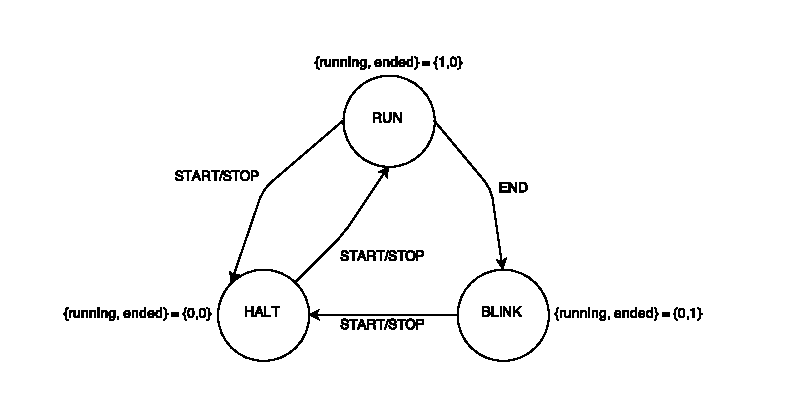
\includegraphics{state_diagram.pdf}
\caption[Diagram przejść pomiędzy trybami timera.]{Diagram przejść
pomiędzy trybami timera. \startstop\ oznacza zdarzenie naciśnięcia
przycisku \startstop , \texttt{END} oznacza zdarzenie zakończenia
zliczania.}
\label{state_diagram}
\end{figure}
\subsection{Symulacja w Multisimie.}
\subsection{Implementacja w HDL.}
Zaimplementowaliśmy powyższy schemat w Verilogu. Sygnały
\startstop\ oraz \texttt{END} doprowadzone są do układu
odpowiednio poprzez wejścia: \texttt{btn} i
\texttt{end\textunderscore}. Na wyjście podawany jest stan
przerzutników \texttt{running} i \texttt{ended}.

\lstinputlisting[title=\texttt{mode.v}]{mode.v}
\section{Dekoder BCD na wyświetlacz 7-segmentowy (\bcdtoseg).}
\subsection{Opis układu.}
Aby użytkownik mógł widzieć stan timera na wyświetlaczu LED,
niezbędne jest \emph{zdekodowanie} sygnału pochodzącego od
liczników, w których cyfry pamiętane są w formacie BCD (Binary
Coded Decimal), na odpowiednie wejścia wyświetlacza 7-segmentowego.
W tym celu zbudowaliśmy układ, który nazwaliśmy \emph{Dekoderem
BCD na wyświetlacz 7-segmentowy}.

Dekoder jest układem \emph{kombinacyjnym}. To oznacza, że sygnał na
wyjściu zależy tylko i wyłącznie od sygnału na wejściu, w
odróżnieniu od układów \emph{sekwencyjnych}. Stan każdego wyjścia
jest opisany funkcją bool'owską, które realizowane są za pomocą
bramek logicznych.

\begin{table}[h] \caption{Tabela stanów logicznych} \label{decoder-table} \centering
\begin{tabular}{|c|cccc|ccccccc|} 
\hline 
& \multicolumn{4}{c|}{BCD} & \multicolumn{7}{c|}{7 segmentowy} \\
N  & Q3   & Q2   & Q1   & Q0  & G   & F  & E  & D  & C  & B  & A  \\ \hline
0  & 0    & 0    & 0    & 0   & 0   & 1  & 1  & 1  & 1  & 1  & 1  \\
1  & 0    & 0    & 0    & 1   & 0   & 0  & 0  & 0  & 1  & 1  & 0  \\
2  & 0    & 0    & 1    & 0   & 1   & 0  & 1  & 1  & 0  & 1  & 1  \\
3  & 0    & 0    & 1    & 1   & 1   & 0  & 0  & 1  & 1  & 1  & 1  \\
4  & 0    & 1    & 0    & 0   & 1   & 1  & 0  & 0  & 1  & 1  & 0  \\
5  & 0    & 1    & 0    & 1   & 1   & 1  & 0  & 1  & 1  & 0  & 1  \\
6  & 0    & 1    & 1    & 0   & 1   & 1  & 1  & 1  & 1  & 0  & 1  \\
7  & 0    & 1    & 1    & 1   & 0   & 0  & 0  & 0  & 1  & 1  & 1  \\
8  & 1    & 0    & 0    & 0   & 1   & 1  & 1  & 1  & 1  & 1  & 1  \\
9  & 1    & 0    & 0    & 1   & 1   & 1  & 0  & 1  & 1  & 1  & 1  \\
10 & 1    & 0    & 1    & 0   & x   & x  & x  & x  & x  & x  & x  \\
11 & 1    & 0    & 1    & 1   & x   & x  & x  & x  & x  & x  & x  \\
12 & 1    & 1    & 0    & 0   & x   & x  & x  & x  & x  & x  & x  \\
13 & 1    & 1    & 0    & 1   & x   & x  & x  & x  & x  & x  & x  \\
14 & 1    & 1    & 1    & 0   & x   & x  & x  & x  & x  & x  & x  \\
15 & 1    & 1    & 1    & 1   & x   & x  & x  & x  & x  & x  & x  \\ \hline
\end{tabular}
\end{table}

\begin{Karnaugh}
\path (name) node {G}; \contingut{0,0,1,1,1,1,1,0,1,1,x,x,x,x,x,x}
\grp{12}{10}{orange}
\grp{2}{10}{green}
\grp{4}{13}{purple}
\grph{3}{10}{blue}
\end{Karnaugh}
%
\begin{Karnaugh}
\path (name) node {F}; \contingut{1,0,0,0,1,1,1,0,1,1,x,x,x,x,x,x}
\grp{0}{8}{green}
\grp{12}{10}{orange}
\grp{4}{13}{purple}
\grpv{4}{14}{blue}
\end{Karnaugh}

\begin{Karnaugh}
\path (name) node {E}; \contingut{1,0,1,0,0,0,1,0,1,0,x,x,x,x,x,x}
\grp{1}{11}{orange}
\grp{4}{13}{green}
\end{Karnaugh}
%
\begin{Karnaugh}
\path (name) node {D}; \contingut{1,0,1,1,0,1,1,0,1,1,x,x,x,x,x,x}
\end{Karnaugh}

\begin{Karnaugh}
\path (name) node {C}; \contingut{1,1,0,1,1,1,1,1,1,1,x,x,x,x,x,x}
\end{Karnaugh}
%    
\begin{Karnaugh}
\path (name) node {B}; \contingut{1,1,1,1,1,0,0,1,1,1,x,x,x,x,x,x}
\end{Karnaugh}

\begin{Karnaugh}
\path (name) node {A}; \contingut{1,0,1,1,0,1,1,1,1,1,x,x,x,x,x,x}
\end{Karnaugh}    

\subsection{Symulacja w Multisimie.}
\subsection{Implementacja w HDL.}
Aby zaimplementować dekoder w Verilogu wystarczy podać, jakiego
zestawu stanów na wyjściu oczekujemy dla każdego zestawu stanów na
wejściu. Kompilator automatycznie będzie się starał zoptymalizować
układ bramek logicznych realizujący podaną w ten sposób
\emph{tabelę prawdy}.

\lstinputlisting[title=\bcdtoseg .v]{bcd_to_7seg.v}

\end{document}
